\documentclass[a4paper,11pt,fleqn]{jarticle}
\usepackage[dvipdfmx]{graphicx}
\usepackage{float}
\usepackage{amsmath}
\usepackage{fancyhdr}

\def \vec#1{\mbox{\boldmath $#1$}} %ベクトルマクロ
\def \bun#1#2{\left(\frac{#1}{#2}\right)} %括弧つき分数マクロ
\def \rot{\nabla \times} %rot
\def \div{\nabla \cdot} %div
\def \intt{\int\!\!\!\int} %2重積分
\def \inttt{\int\!\!\!\int\!\!\!\int} %3重積分

% ページレイアウト
\setlength{\topmargin}{10mm}
  \addtolength{\topmargin}{-1in}
\setlength{\oddsidemargin}{30mm}
  \addtolength{\oddsidemargin}{-1in}
\setlength{\textwidth}{150mm}
\setlength{\textheight}{250mm}
\setlength{\headsep}{2zw}
\setlength{\headheight}{2zw}
\setlength{\topskip}{15mm}
\linespread{1.0}

% サブセクションを1.,2.にする設定
\renewcommand{\thesubsection}{\arabic{subsection}.}

% サブサブセクションを(1),(2)にする設定
\renewcommand{\thesubsubsection}{(\arabic{subsubsection})}

% 大問2の3番目の計算式のラベルを(2.3)にする設定
% 計算式の参照には\eqref{eq:hoge}を使う
\makeatletter
  \renewcommand{\theequation}{\arabic{subsection}.\arabic{equation}}
  \@addtoreset{equation}{subsection}
\pagestyle{fancy}
% ヘッダーの設定
  \lhead[物理数学 2016.04.14]{\leftmark}
  \rhead[\leftmark]{物理数学 2016.04.14}
\renewcommand{\headrulewidth}{0pt}
\makeatother


\begin{document}


\begin{center}
\begin{Large}
演習問題その4 解答例
\end{Large}
\end{center}

\subsection{}
デカルト座標系$(x,y,z)$と円柱座標系$(\rho ,\phi ,z)$の間の座標変換を考える。
\subsubsection{$(x,y,z)を(\rho ,\phi ,z)を用いて表せ。また、(\rho ,\phi ,z)を(x,y,z)を用いて表せ。$}
\subsubsection{$\vec{e}_{\rho},\vec{e}_{\phi},\vec{e}_zを\vec{e}_x,\vec{e}_y,\vec{e}_zを用いて表せ。また、\vec{e}_x,\vec{e}_y,\vec{e}_zを\vec{e}_{\rho},\vec{e}_{\phi},\vec{e}_zを用いて表せ。$}
(解答例)
\begin{eqnarray*}
x=\rho\cos\phi,~y=\rho\sin\phi,~z=z
\end{eqnarray*}
\begin{eqnarray*}
\rho =\sqrt{x^2+y^2},~\phi =\tan^{-1}\left(\frac{y}{x}\right),~z=z
\end{eqnarray*}

$e_z$はデカルト座標でも円筒座標でも共通である。($\vec{e}_\rho$, $\vec{e}_\phi$)と$(\vec{e}_x,\vec{e}_y)$は平面内を$\phi$だけ回転させたものであるので、
\begin{eqnarray}
  \left(
    \begin{array}{c}
      \vec{e}_\rho \\
      \vec{e}_\phi \\
    \end{array}
    \right)
    =
      \left(
    \begin{array}{cc}
      \cos\phi & \sin\phi \\
      -\sin\phi & \cos\phi \\
    \end{array}
    \right)
      \left(
    \begin{array}{c}
      \vec{e}_x \\
      \vec{e}_y \\
    \end{array}
    \right) \label{eq:cy}
\end{eqnarray}
よって$\vec{e}_\rho=\cos\phi\vec{e}_x+\sin\phi\vec{e}_y$, $\vec{e}_\phi=-\sin\phi \vec{e}_x+\cos\phi\vec{e}_y$, $\vec{e}_z=\vec{e}_z$.\\
\\
いっぽう、式(\ref{eq:cy})両辺に逆行列をかける事で、\\
$\vec{e}_x=\cos\phi\vec{e}_\rho-\sin\phi\vec{e}_\phi$, $\vec{e}_y=\sin\phi\vec{e}_\rho+\cos\phi\vec{e}_\phi$を得る。\\

\subsubsection{$デカルト座標系で\vec{A}=z\vec{e}_x-2x\vec{e}_y+y\vec{e}_zと表されるベクトル\vec{A}を円柱座標系で表せ。$}
(解答例)
\begin{eqnarray*}
\vec{A}&=&z(\cos\phi\vec{e}_\rho-\sin\phi\vec{e}_\phi)-2\rho\cos\phi(\sin\phi\vec{e}_\rho+\cos\phi\vec{e}_\phi)+\rho\sin\phi\vec{e}_z\\
&=&(z\cos\phi-2\rho\cos\phi\sin\phi)\vec{e}_\rho-(z\sin\phi+2\rho{\cos}^2\phi)\vec{e}_\phi+\rho\sin\phi\vec{e}_z
\end{eqnarray*}


\newpage
\subsection{}
デカルト座標系$(x,y,z)$と極座標系$(r ,\theta ,\phi)$の間の座標変換を考える。
\subsubsection{$(x,y,z)を(r ,\theta ,\phi )を用いて表せ。また、(r ,\theta ,\phi )を(x,y,z)を用いて表せ。$}
\subsubsection{$\vec{e}_{r},\vec{e}_{\theta},\vec{e}_{\phi}を\vec{e}_x,\vec{e}_y,\vec{e}_zを用いて表せ。また、\vec{e}_x,\vec{e}_y,\vec{e}_zを\vec{e}_{r},\vec{e}_{\theta},\vec{e}_{\phi}を用いて表せ。$}
(解答例)
\begin{eqnarray*}
x=r\sin\theta\cos\phi ,~y=r\sin\theta\sin\phi, ~z=r\cos\theta
\end{eqnarray*}
\begin{eqnarray*}
r=\sqrt{x^2+y^2+z^2},~
\theta =\tan^{-1}\left(\frac{\sqrt{x^2+y^2}}{z}\right),~
\phi =\tan^{-1}\left(\frac{y}{x}\right)
\end{eqnarray*}
$\vec{r}=x\vec{e}_x+y\vec{e}_y+z\vec{e}_z=(x,y,z)$とすると、極座標系の基底ベクトルは以下のように与えられる。
\begin{eqnarray*}
\vec{e}_r=\frac{\partial \vec{r}}{\partial r}/|\frac{\partial \vec{r}}{\partial r}|
,~\vec{e}_{\theta}=\frac{\partial \vec{r}}{\partial \theta}/|\frac{\partial \vec{r}}{\partial \theta}|
,~\vec{e}_{\phi}=\frac{\partial \vec{r}}{\partial \phi}/|\frac{\partial \vec{r}}{\partial \phi}|
\end{eqnarray*}
\begin{eqnarray*}
\frac{\partial \vec{r}}{\partial r}=(\sin\theta\cos\phi ,\sin\theta\sin\phi ,\cos\theta ),~|\frac{\partial \vec{r}}{\partial r}|=1\\
\frac{\partial \vec{r}}{\partial \theta}=(r\cos\theta\cos\phi ,r\cos\theta\sin\phi ,-r\sin\theta ),~|\frac{\partial \vec{r}}{\partial \theta}|=r\\
\frac{\partial \vec{r}}{\partial \phi}=(-r\sin\theta\sin\phi ,r\sin\theta\cos\phi ,0),~|\frac{\partial \vec{r}}{\partial \phi}|=r\sin\theta
\end{eqnarray*}
よって、

\begin{eqnarray*}
      \left(
    \begin{array}{c}
      \vec{e}_r \\
      \vec{e}_\theta \\
      \vec{e}_\phi\\
    \end{array}
    \right)
  &=& 
     \left(
    \begin{array}{ccc}
    \sin\theta\cos\phi & \sin\theta\sin\phi & \cos\theta \\
    \cos\theta\cos\phi & \sin\phi\cos\theta & -\sin\theta\\
    -\sin\phi & \cos\phi & 0
    \end{array}
    \right)
        \left(
    \begin{array}{c}
      \vec{e}_x \\
      \vec{e}_y \\
      \vec{e}_z\\
    \end{array}
    \right)
\end{eqnarray*}
逆行列をかけて、
\begin{eqnarray*}
       \left(
    \begin{array}{c}
      \vec{e}_x \\
      \vec{e}_y \\
      \vec{e}_z\\
    \end{array}
    \right)
    ~=~
         \left(
    \begin{array}{ccc}
    \sin\theta\cos\phi &  \cos\theta\cos\phi &-\sin\phi  \\
   \sin\theta\sin\phi & \sin\phi\cos\theta &\cos\phi  \\
    \cos\theta & -\sin\theta& 0
    \end{array}
    \right)
            \left(
    \begin{array}{c}
      \vec{e}_r \\
      \vec{e}_\theta \\
      \vec{e}_\phi\\
    \end{array}
    \right)
\end{eqnarray*}

\newpage
\subsubsection{$極座標系で、\vec{A}=r^2\sin\theta\vec{e}_{\theta}と表されるベクトル\vec{A}をデカルト座標で表せ。$}
(解答例)
\begin{eqnarray*}
{\Vec e}_{\theta}&=&\cos\theta\cos\phi{\Vec e}_{\it x}+\cos\theta\sin\phi{\Vec e}_{\it y}-\sin\theta{\Vec e}_{\it z} 
\end{eqnarray*}
であるので,
\begin{eqnarray*}
{\Vec A}&=&r^2\sin\theta\cos\theta\cos\phi{\Vec e}_{\it x}+r^2\sin\theta\cos\theta\sin\phi{\Vec e}_{\it y}-r^2\sin^2\theta{\Vec e}_{\it z}  \\
&=&(r\sin\theta\cos\phi)(r\cos\theta){\Vec e}_{\it x}+(r\cos\theta)(r\sin\theta\sin\phi){\Vec e}_{\it y}-(r^2-r^2\cos^2\theta){\Vec e}_{\it z}  \\
&=&xz{\Vec e}_{\it x}+yz{\Vec e}_{\it y}-(x^2+y^2){\Vec e}_{\it z}.
\end{eqnarray*}


\vspace{20mm}
\subsection{}
$f=x+2y+z$とする。極座標系での$\nabla f$をそれぞれ求めよ。
\begin{eqnarray*}
(解答例)
\end{eqnarray*}
$f$を球座標系で書きなおすと、
\begin{eqnarray*}
f=r\sin\theta\cos\phi+2r\sin\theta\sin\phi+r\cos\theta
\end{eqnarray*}
よって、
\begin{eqnarray*}
\nabla f&=&\frac{\partial f}{\partial r}{\Vec e}_{\it r}+\frac{1}{r}\frac{\partial f}{\partial \theta}{\Vec e}_{\theta}
+\frac{1}{r\sin\theta}\frac{\partial f}{\partial \phi}{\Vec e}_{\it \phi} \\
&=&(\sin\theta\cos\phi+2\sin\theta\sin\phi+\cos\theta){\Vec e}_{\it r} \\
&&+(\cos\theta\cos\phi+2\cos\theta\sin\phi-\sin\theta){\Vec e}_{\theta} \\
&&+(2\cos\phi-\sin\phi){\Vec e}_{\phi}
\end{eqnarray*}


\newpage
\subsection{}
円柱座標系$(\rho ,\phi ,z)$で$\vec{a}=\rho\cos\phi\vec{e}_{\rho}-z\sin\phi\vec{e}_{\phi}+\rho z\vec{e}_z$と表されるベクトル$\vec{a}$について、$\nabla\cdot\vec{a},~\nabla\times\vec{a}$をそれぞれ求めよ。
\begin{eqnarray*}
(解答例)
\end{eqnarray*}
\begin{eqnarray*}
\vec{a} ~=~ a_{\rho}\vec{e}_{\rho}+a_{\phi}\vec{e}_\phi +a_z\vec{e}_z
\end{eqnarray*}
とおくと、
\begin{eqnarray*}
\div\vec{a} &=& \frac{1}{\rho}\frac{\partial}{\partial \rho}(\rho a_{\rho})+\frac{1}{\rho}\frac{\partial a_{\phi}}{\partial \phi}+\frac{\partial a_z}{\partial z}\\
\rot\vec{a} &=& \left(\frac{1}{\rho}\frac{\partial a_z}{\partial \phi}-\frac{\partial a_{\phi}}{\partial z},~\frac{\partial a_{\rho}}{\partial z}-\frac{\partial a_z}{\partial \rho},~\frac{1}{\rho}\frac{\partial (\rho a_{\phi})}{\partial \rho}-\frac{1}{\rho}\frac{\partial a_{\rho}}{\partial \phi}\right)
\end{eqnarray*}
であるので、具体的に計算することにより、
\begin{eqnarray*}
\div\vec{a} &=& \cos\phi\left(2-\frac{z}{\rho}\right)+\rho \\
\rot\vec{a} &=& \sin\phi\vec{e}_{\rho}-z\vec{e}_{\phi}+\sin\phi\left(1-\frac{z}{\rho}\right)\vec{e}_z
\end{eqnarray*}

\newpage
\subsection{}
円柱座標系$(\vec{e}_{\rho},\vec{e}_{\phi},\vec{e}_z)$について、以下の問いに答えよ。
\subsubsection{}
基底ベクトルの時間微分が$\frac{d}{d t}\vec{e}_{\rho}=\dot{\phi}\vec{e}_{\phi},~\frac{d}{d t}\vec{e}_{\phi}=-\dot{\phi}\vec{e}_{\rho}$であることを示せ。

\begin{eqnarray*}
(解答例)
\end{eqnarray*}
\begin{eqnarray*}
\frac{d}{dt}\vec{e}_\rho&=&\frac{d}{dt}(\cos\phi\vec{e}_x+\sin\phi\vec{e}_y)\\
&=&\dot{\phi}(-\sin\phi\vec{e}_x+\cos\phi\vec{e}_y)=\dot{\phi}\vec{e}_\phi
\end{eqnarray*}
\begin{eqnarray*}
\frac{d}{dt}\vec{e}_\phi&=&\frac{d}{dt}(-\sin\phi\vec{e}_x+\cos\phi\vec{e}_y)\\
&=&\dot{\phi}(-\cos\phi\vec{e}_x-\sin\phi\vec{e}_y)=-\dot{\phi}\vec{e}_\rho
\end{eqnarray*}

\vspace{20mm}
\subsubsection{}
質点の速度$\vec{v}$、加速度$\vec{a}$を円筒座標系で表せ。
\begin{eqnarray*}
(解答例)
\end{eqnarray*}
粒子の位置ベクトル$\vec{r}=x\vec{e}_x+y\vec{e}_y+z\vec{e}_z$を円柱座標系に書き直すと、\\
$\vec{r}=\rho\vec{e}_\rho+z\vec{e}_z$と書ける。これを時間微分して、
\begin{eqnarray*}
\vec{v}&=&\frac{d\vec{r}}{dt}=\frac{d\rho}{dt}\vec{e}_\rho+\rho\frac{d\vec{e}_\rho}{dt}+\frac{dz}{dt}\vec{e}_z\\
&=&\dot{\rho}\vec{e}_\rho+\rho\dot{\phi}\vec{e}_\phi+\dot{z}\vec{e}_z
\end{eqnarray*}
\begin{eqnarray*}
\vec{a}&=&\frac{d\vec{v}}{dt}=\frac{d}{dt}(\dot{\rho}\vec{e}_\rho+\rho\dot{\phi}\vec{e}_\phi+\dot{z}\vec{e}_z)\\
&=&(\ddot{\rho}-\rho\dot{\phi}^2)\vec{e}_\rho+(\rho\ddot{\phi}+2\dot{\rho}\dot{\phi})\vec{e}_\phi+\ddot{z}\vec{e}_z
\end{eqnarray*}

\newpage
\subsection{}
以下の問いに答えよ。
\subsubsection{$\vec{a}=(3x^2+y^2)\vec{e}_x+2xy\vec{e}_y+z^2\vec{e}_zであるとき、x=r\cos\phi ,~y=r\sin\phi ,~z=zとして次式を媒介変数r,\phi ,zで表せ(\vec{a}やd\vec{r}を円柱座標系の基底ベクトルを用いて表す必要はない)$}
\begin{center}
$\int_C \vec{a}\cdot d\vec{r}$
\end{center}
(解答例)
\begin{eqnarray*}
\vec{a} &=& (3x^2+y^2)\vec{e}_x+2xy\vec{e}_y+z^2\vec{e}_z\\
        &=& \lbrace 3(r\cos\phi )^2+(r\sin\phi )^2 \rbrace\vec{e}_x+2(r\cos\phi )(r\sin\phi)\vec{e}_y+z^2\vec{e}_z\\
        &=& (r^2+2r^2{\cos}^2\phi )\vec{e}_x+2r^2\sin\phi\cos\phi\vec{e}_y+z^2\vec{e}_z
\end{eqnarray*}
${\rm d}\vec{r}$は、${\rm d}x=\cos\phi{\rm d}r -\rho\sin\phi{\rm d}\phi ,~{\rm d}y=\sin\phi{\rm d}r +r\cos\phi{\rm d}\phi ,~{\rm d}z={\rm d}z$
これらを用いて計算することで以下が得られる。
\begin{eqnarray*}
\int_C \vec{a}\cdot d\vec{r} = \int_C (3r^2\cos\phi{\rm d}r- r^3\sin\phi{\rm d}\phi +z^2{\rm d}z)
\end{eqnarray*}

\vspace{20mm}
\subsubsection{$z=0上の平面において、Cが半径3の半円の弧を描くとき(1)の線積分の値を求めよ(つまり、Cはr=3=一定,\phi :[0\rightarrow\pi ]となる)$}

(解答例)\\
$r=3,~z=0,~{\rm d}r=0,~{\rm d}z=0$として、(1)の値は以下のようになる。
\begin{eqnarray*}
\int_C \vec{a}\cdot d\vec{r}
&=& \int_C (3r^2\cos\phi{\rm d}r- r^3\sin\phi{\rm d}\phi +z^2{\rm d}z)\\
&=& \int_C (3\cdot3^2\cos\phi\cdot 0-3^3\sin\phi{\rm d}\phi +0)\\
&=& \int_0^\pi (-27\sin\phi ){\rm d}\phi =-54.
\end{eqnarray*}

\newpage
\subsection{}
$\vec{b}=-z\vec{e}_{x}-3x^2y\vec{e}_{y}+2x^2y^2\vec{e}_{z}$とする.図のような立方体の面EFGHを除く5つの面を$S$とし,閉曲線E→H→G→F→Eを$C$とするとき,$\int_S (\nabla\times \vec{b})\cdot \mathrm{d}\vec{S}$と$\int_C \vec{b} \cdot \mathrm{d}\vec r$を計算することにより,ストークスの定理が成り立っていることを確かめよ.
\begin{center}
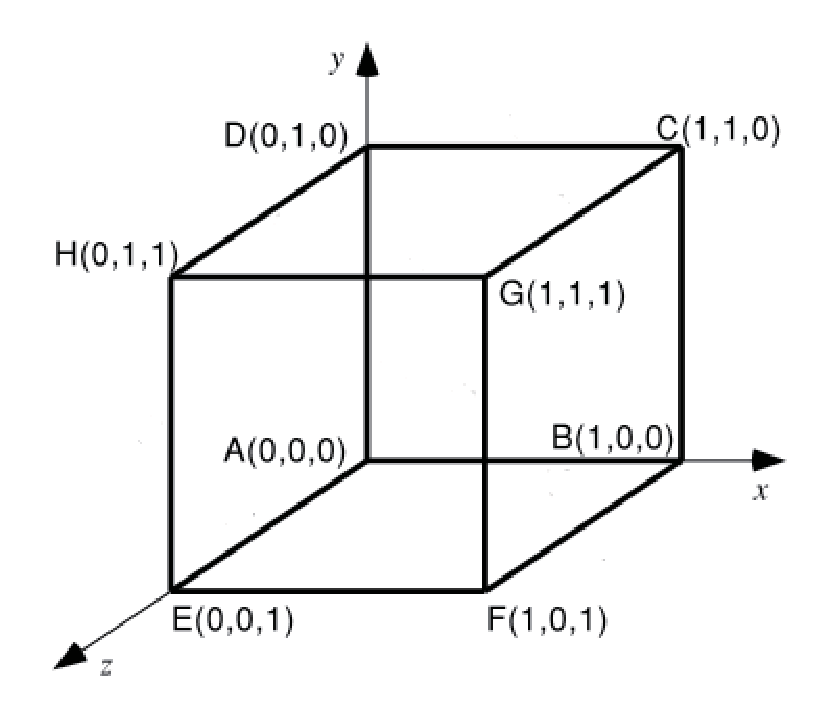
\includegraphics[width=.4\textwidth,bb=19 19 400 340]{5fig/rippou.eps}
\label{rippou}
\end{center}

(解答例)

まず面積分を計算する.$\rot \vec b=4x^2y\vec{e}_{x}-(1+4xy^2)\vec{e}_{y}-6xy\vec{e}_{z}$であるので,
立方体の各面について$\left(\nabla \times \vec{b} \right) \cdot \mathrm{d}\vec{S}$を考えると,\\[8pt]
%%%%
面ABCD : $z=0,\; \mathrm{d}\vec{S}=-\vec{e}_{z}\mathrm{d}x \mathrm{d}y \ \ 
\Rightarrow \left(\nabla \times \vec{b} \right) \cdot \mathrm{d}\vec{S} = 6xy \mathrm{d}x \mathrm{d}y$,\\
%%%%
面AEFB : $y=0,\; \mathrm{d}\vec{S}=-\vec{e}_{y}\mathrm{d}z \mathrm{d}x \ \ 
\Rightarrow \left(\nabla \times \vec{b} \right) \cdot \mathrm{d}\vec{S} = \mathrm{d}z \mathrm{d}x$,\\
%%%%
面ADHE : $x=0,\; \mathrm{d}\vec{S}=-\vec{e}_{x}\mathrm{d}y \mathrm{d}z \ \ 
\Rightarrow \left(\nabla \times \vec{b} \right) \cdot \mathrm{d}\vec{S} = 0$,\\
%%%%
面BCGF : $x=1,\; \mathrm{d}\vec{S}=\vec{e}_{x}\mathrm{d}y \mathrm{d}z \ \ 
\Rightarrow \left(\nabla \times \vec{b} \right) \cdot \mathrm{d}\vec{S} = 4y \mathrm{d}y \mathrm{d}z$,\\
%%%%
面CDHG : $y=1,\; \mathrm{d}\vec{S}=\vec{e}_{y}\mathrm{d}z \mathrm{d}x \ \ 
\Rightarrow \left(\nabla \times \vec{b} \right) \cdot \mathrm{d}\vec{S} = -\left(4x+1 \right) \mathrm{d}z \mathrm{d}x$.\\[8pt]
%%%%
従って,
%
\begin{eqnarray*}
\intt_{S} \left(\nabla \times \vec{b} \right) \cdot \mathrm{d}\vec{S} &=&
\intt_{\mathrm{ABCD}}\left(\nabla \times \vec{b} \right) \cdot \mathrm{d}\vec{S}
+  \intt_{\mathrm{AEFB}}\left(\nabla \times \vec{b} \right) \cdot \mathrm{d}\vec{S}\\
&+& \intt_{\mathrm{BCGF}}\left(\nabla \times \vec{b} \right) \cdot \mathrm{d}\vec{S}
+  \intt_{\mathrm{CDHF}}\left(\nabla \times \vec{b} \right) \cdot \mathrm{d}\vec{S}\\
%
&=&\int_0^1\int_0^1 6xy \mathrm{d}x \mathrm{d}y + \int_0^1\int_0^1\mathrm{d}z \mathrm{d}x
+ \int_0^1\int_0^1 4y \mathrm{d}y \mathrm{d}z - \int_0^1\int_0^1 \left(4x+1 \right) \mathrm{d}z \mathrm{d}x \\
&=&\frac{3}{2}+1+2-3=\frac{3}{2}.
\end{eqnarray*}
%
次に線積分を計算する.
媒介変数$t \ (0\le t\le 1$)を用いると各経路における$\vec{b}\cdot \mathrm{d}\vec{r}$は,\\[8pt]
E→H \ : \ $\vec{r}=t \vec{e}_{y}+\vec{e}_{z}, \ \mathrm{d}\vec{r}=\mathrm{d}t \vec{e}_{y} \Rightarrow \vec{b}\cdot \mathrm{d}\vec{r}=0$,\\
H→G \ : \ $\vec{r}=t \vec{e}_{x}+\vec{e}_{y}+\vec{e}_{z}, \ \mathrm{d}\vec{r}=\mathrm{d}t \vec{e}_{x} \Rightarrow \vec{b}\cdot \mathrm{d}\vec{r}=-\mathrm{d}t$,\\
G→F \ : \ $\vec{r}= \vec{e}_{x}+(1-t)\vec{e}_{y}+\vec{e}_{z}, \ \mathrm{d}\vec{r}=-\mathrm{d}t \vec{e}_{y} \Rightarrow \vec{b}\cdot \mathrm{d}\vec{r}=3(1-t)\mathrm{d}t$,\\
F→E \ : \ $\vec{r}=(1-t) \vec{e}_{x}+\vec{e}_{z}, \ \mathrm{d}\vec{r}=-\mathrm{d}t \vec{e}_{x} \Rightarrow \vec{b}\cdot \mathrm{d}\vec{r}=\mathrm{d}t$.\\[8pt]
よって
\begin{eqnarray*}
\oint_C\vec b \cdot \mathrm{d}\vec{r} &=& \int_{\rm H\to\rm G}\vec b \cdot \mathrm{d}\vec{r} 
 + \int_{\rm G\to\rm F}\vec b \cdot \mathrm{d}\vec{r}+\int_{\rm F\to\rm E}\vec b \cdot \mathrm{d}\vec{r}\\
 &=& -\int_0^1 \mathrm{d}t + \int_0^1 \mathrm{d}t + 3\int_0^1 (1-t)\mathrm{d}t\\
 &=& 3 \left[t-\frac{t^2}{2} \right]^1_0=\frac{3}{2}.
\end{eqnarray*}

以上より,
$\intt_S(\rot \vec b)\cdot \mathrm{d}\vec{S}=\oint_C\vec b \cdot \mathrm{d}\vec{r}=3/2$なのでストークスの定理は成り立っている.\\

\subsection{}
放物面$z=1-(x^2+y^2)$のうち,$z\ge 0$の領域を$S$とする.
$\vec{a}=-2y \vec{e}_{x}+ x \vec{e}_{y}+ z \vec{e}_{z}$とするとき,$\int_S(\nabla\times \vec{a})\cdot \mathrm{d}\vec{S}$を計算せよ.ただし,$d\vec{S}$の向きは$+z$方向とする。\\
(ヒント:面積分しない)

(解答例)\\[10pt]
放物面と平面$z=0$との交線である円$x^2+y^2=1$を反時計回りに回る経路を$C$とする.
媒介変数$t \ (0\le t\le 2\pi)$を用いて,$C$上の位置ベクトル$\vec{r}$を$\vec{r}=\cos t \vec{e}_{x}+\sin t \vec{e}_{y}$と表すとき,
$\vec{a}=-2\sin t \vec{e}_{x}+\cos t \vec{e}_{y}, \ \mathrm{d}\vec{r}=(-\sin t \vec{e}_{x}+\cos t \vec{e}_{y})\mathrm{d}t$
となるので,
%
\begin{eqnarray*}
\label{a}
\vec{a}\cdot \mathrm{d}\vec{r}=(2\sin^2 t + cos^2 t)\mathrm{d}t = (1+\sin^2 t)\mathrm{d}t.
\end{eqnarray*}
%
ストークスの定理より
\begin{eqnarray*}
\intt_{S} (\nabla \times \vec{a})\cdot \mathrm{d}\vec{S}&=&\oint_C \vec{a}\cdot \mathrm{d}\vec{r}\\[10pt]
&=& \int_{0}^{2\pi}(1+\sin^2 t)\mathrm{d}t \\[10pt]
&=& \int_{0}^{2\pi}\frac{3-\cos 2t}{2}\mathrm{d}t\\[12pt]
&=& 3\pi.
\end{eqnarray*}

\subsection{}
ある場から物体に働く力$\vec{F}$が、スカラー場$\phi$を用いて$\vec{F}=-\nabla\phi$と書けるとき、この力$\vec{F}$が保存力であることを示せ。ただし、保存力とは、任意の2点間を移動するときになされる仕事が経路に依らないような力のことである。\\
(ヒント:任意のスカラー場$\phi$に対して$\nabla\times (\nabla\phi )$をとると...?)

(解答例)\\[10pt]
\begin{center}
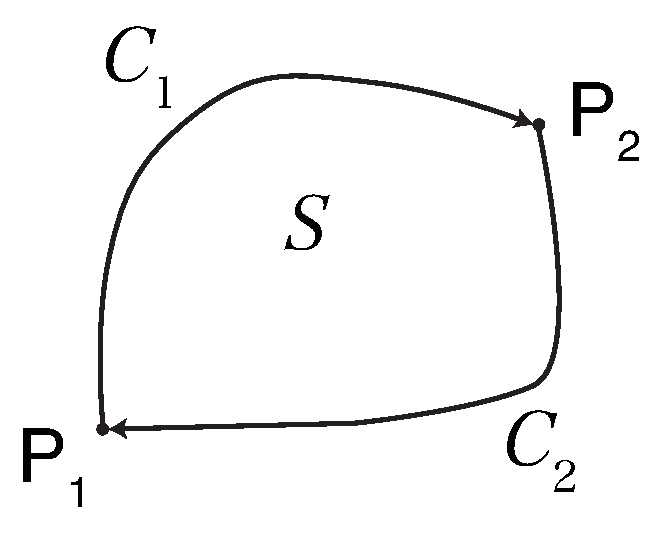
\includegraphics[width=.3\textwidth]{5fig/pote.eps}
\end{center}

図のような空間中の任意の異なる2点$\mathrm{P}_1, \mathrm{P}_2$と,2点をつなぐ任意の異なる2経路$C_1 \ (\rm P_1\to\rm P_2)$,$C_2 \ (\rm P_2\to\rm P_1)$を考え,$C_1$と$C_2$に囲まれた領域を$S$とする.\\
いま,質点が経路$C_1+C_2$を移動する間に場からなされる仕事は,
ストークスの定理より
\begin{eqnarray*}
\oint_{C_1+C_2} \vec{F}\cdot \mathrm{d}\vec{r}&=&\intt_{S} (\nabla \times \vec{F})\cdot \mathrm{d}\vec{S}\\
&=&-\intt_{S} (\nabla \times \nabla \phi)\cdot \mathrm{d}\vec{S}\\[12pt]
&=& 0 \ \ \  (任意のスカラー場 \phi に対して \nabla \times (\nabla \phi)=0)
\end{eqnarray*}
となる.これより,
%
\begin{eqnarray*}
\label{a}
\oint_{C_1+C_2} \vec{F}\cdot \mathrm{d}\vec{r}&=&\int_{C_1}\vec{F}\cdot \mathrm{d}\vec{r} + \int_{C_2}\vec{F}\cdot \mathrm{d}\vec{r}=0,\\
\end{eqnarray*}
\begin{eqnarray*}
&\Leftrightarrow& \int_{C_1}\vec{F}\cdot \mathrm{d}\vec{r}=-\int_{C_2}\vec{F}\cdot \mathrm{d}\vec{r},\\[10pt]
\int_{C_1}\vec{F}\cdot \mathrm{d}\vec{r}=\int_{-C_2}\vec{F}\cdot \mathrm{d}\vec{r}.
\end{eqnarray*}
%
ここで,経路$-C_2$は$\rm P_1と\rm P_2$を結ぶ$C_1$とは異なる経路である.
上式が任意の$C_1$,$C_2$で成り立つので,任意の点$\mathrm{P}_1$から$\mathrm{P}_2$までを移動する間に場からなされる仕事は,
その経路によらない.従って$\vec{F}$は保存力である.\\

\newpage
\subsection{$+\alpha$問題}
任意の直交曲線座標系(円柱座標系や球座標系など)$q_1,q_2,q_3$における$\nabla{f}$の表記が以下の通りであることを示したい。
\begin{eqnarray*}
\nabla{f}=\frac{\partial{f}}{h_1\partial{q_1}}\vec{e}_1+\frac{\partial{f}}{h_2\partial{q_2}}\vec{e}_2+\frac{\partial{f}}{h_3\partial{q_3}}\vec{e}_3
\end{eqnarray*}
ただし、$\delta{\vec{r}}=\delta{x}\vec{e}_x+\delta{y}\vec{e}_y+\delta{z}\vec{e}_z=h_1\delta{q_1}\vec{e}_1+h_2\delta{q_2}\vec{e}_2+h_3\delta{q_3}\vec{e}_3$である。
\subsubsection{$まずデカルト座標系において(x,y,z)\rightarrow(x+\delta{x},y+\delta{y},z+\delta{z})となったときのfの変化量\delta fを求めることにより、\nabla f\cdot\delta\vec{r}となることを示せ。$}

(解答例)
\begin{eqnarray*}
\delta{f}&=&f(x+\delta{x},y+\delta{y},z+\delta{z})-f(x,y,z)\\
&=&\frac{\partial{f}}{\partial{x}}\delta{x}+\frac{\partial{f}}{\partial{y}}\delta{y}+\frac{\partial{f}}{\partial{z}}\delta{z}\\
&=&\frac{\partial{f}}{\partial{x}}\vec{e}_x\cdot\delta{x}\vec{e}_x+\frac{\partial{f}}{\partial{y}}\vec{e}_y\cdot\delta{y}\vec{e}_y+\frac{\partial{f}}{\partial{z}}\vec{e}_z\cdot\delta{z}\vec{e}_z
\end{eqnarray*}
ここで、$\nabla=\frac{\partial}{\partial{x}}\vec{e}_x+\frac{\partial}{\partial{y}}\vec{e}_y+\frac{\partial}{\partial{z}}\vec{e}_z$, $\delta\vec{s}=\delta{x}\vec{e}_x+\delta{y}\vec{e}_y+\delta{z}\vec{e}_z$
より以下のようになる。
\begin{eqnarray*}
\delta{f}=\nabla{f}\cdot\delta\vec{s}.
\end{eqnarray*}


\subsubsection{$次に任意の直交曲線座標系で(q_1,q_2,q_3)\rightarrow(q_1+\delta{q_1},q_2+\delta{q_2},q_3+\delta{q_3})となったときのfの変化量\delta fを求め、題意を示せ。$}

(解答例)
\begin{eqnarray*}
\delta{f}&=&f(q_1+\delta{q_1},q_2+\delta{q_2},q_3+\delta{q_3})-f(q_1,q_2,q_3)\\
&=&\frac{\partial{f}}{\partial{q_1}}\delta{q_1}+\frac{\partial{f}}{\partial{q_2}}\delta{q_2}+\frac{\partial{f}}{\partial{q_3}}\delta{q_3}\\
&=&\frac{\partial{f}}{h_1\partial{q_1}}(h_1\delta{q_1})+\frac{\partial{f}}{h_2\partial{q_2}}(h_2\delta{q_2})+\frac{\partial{f}}{h_3\partial{q_3}}(h_3\delta{q_3})
\end{eqnarray*}
ここで、$\delta{\vec{r}}=h_1\delta{q_1}\vec{e}_1+h_2\delta{q_2}\vec{e}_2+h_3\delta{q_3}\vec{e}_3$
より以下のようになる。
\begin{eqnarray*}
\delta{f}&=&\frac{\partial{f}}{h_1\partial{q_1}}\vec{e}_1\cdot(h_1\delta{q_1})\vec{e}_1+\frac{\partial{f}}{h_2\partial{y}}\vec{e}_2\cdot(h_2\delta{q_2})\vec{e}_2+\frac{\partial{f}}{h_3\partial{z}}\vec{e}_3\cdot(h_3\delta{q_3})\vec{e}_3\\
&=&\left(\frac{\partial{f}}{h_1\partial{q_1}}\vec{e}_1+\frac{\partial{f}}{h_2\partial{y}}\vec{e}_2+\frac{\partial{f}}{h_3\partial{z}}\vec{e}_3\right)\cdot\delta\vec{s}
\end{eqnarray*}
(1)より$\delta{f}=\nabla{f}\cdot\delta\vec{s}$だったので
\begin{eqnarray*}
\nabla{f}=\frac{\partial{f}}{h_1\partial{q_1}}\vec{e}_1+\frac{\partial{f}}{h_2\partial{q_2}}\vec{e}_2+\frac{\partial{f}}{h_3\partial{q_3}}\vec{e}_3
\end{eqnarray*}
である。よって題意が示された。

\newpage
\subsubsection{$上記の結果を用いて、極座標系における\nabla fを求めよ。$}
補足:$h_i(i=1,2,3)$について、
\begin{eqnarray*}
h_i\delta{q}_i\vec{e}_i=\frac{\partial{x}}{\partial{q_i}}\delta{q}_i\vec{e}_x+\frac{\partial{y}}{\partial{q_i}}\delta{q}_i\vec{e}_y
+\frac{\partial{z}}{\partial{q_i}}\delta{q}_i\vec{e}_z
\end{eqnarray*}
となるので$h_i$は以下のように表せる:
\begin{eqnarray*}
h_i=\sqrt{\left(\frac{\partial{x}}{\partial{q_i}}\right)^2+\left(\frac{\partial{y}}{\partial{q_i}}\right)^2+\left(\frac{\partial{z}}{\partial{q_i}}\right)^2}
\end{eqnarray*}
\begin{eqnarray*}
(解答例)
\end{eqnarray*}
極座標では、$\vec{r}=(x,y,z)=(r\sin\theta\cos\phi ,r\sin\theta\sin\phi ,r\cos\theta)$となる。\\
$q_1=r,~q_2=\theta ,~q_3=\phi$とおけば、$h_r,~h_{\theta},~h_{\phi}$はそれぞれ以下のようになる。

\begin{eqnarray*}
h_r&=&\sqrt{\left(\frac{\partial{x}}{\partial{r}}\right)^2+\left(\frac{\partial{y}}{\partial{r}}\right)^2+\left(\frac{\partial{z}}{\partial{r}}\right)^2}=1\\
h_\theta&=&\sqrt{\left(\frac{\partial{x}}{\partial{\theta}}\right)^2+\left(\frac{\partial{y}}{\partial{\theta}}\right)^2+\left(\frac{\partial{z}}{\partial{\theta}}\right)^2}=r\\
h_{\phi}&=&\sqrt{\left(\frac{\partial{x}}{\partial \phi}\right)^2+\left(\frac{\partial{y}}{\partial  \phi}\right)^2+\left(\frac{\partial \phi}{\partial z}\right)^2}=r\sin\theta
\end{eqnarray*}
よって、$\nabla f$は、
\begin{eqnarray*}
\nabla f ~=~ \frac{\partial f}{\partial r}\vec{e}_r+\frac{1}{r}\frac{\partial f}{\partial \theta}\vec{e}_{\theta}+\frac{1}{r\sin\theta}\frac{\partial f}{\partial \phi}\vec{e}_{\phi}
\end{eqnarray*}

\newpage
\subsubsection{時間が余った人向け}
(3)で求めた、極座標についての$\nabla$を用いて$\Delta f$が以下のように記述できることを示せ。
\begin{eqnarray*}
\Delta f=\frac{1}{r^2}\frac{\partial}{\partial r}\left(r^2\frac{\partial f}{\partial r}\right)+\frac{1}{r^2\sin\theta}\frac{\partial}{\partial \theta}\left(\sin\theta\frac{\partial f}{\partial \theta}\right)+\frac{1}{r^2{\sin}^2\theta}\frac{{\partial}^2 f}{\partial {\phi}^2}
\end{eqnarray*}
補足:\\
$\Delta f=\nabla\cdot (\nabla f).~$極座標の単位ベクトルの座標微分($\frac{\partial}{\partial \phi}\vec{e}_{\theta}$など)はゼロでないことに注意。
\begin{eqnarray*}
(解答例)
\end{eqnarray*}
\begin{eqnarray*}
\Delta f &=& \nabla\cdot (\nabla f)\\
&=& \left( \vec{e}_r\frac{\partial}{\partial r}+\vec{e}_{\theta}\frac{1}{r}\frac{\partial}{\partial \theta}+\vec{e}_{\phi}\frac{1}{r\sin\theta}\frac{\partial}{\partial \phi}\right)\cdot\left(\frac{\partial f}{\partial r}\vec{e}_r+\frac{1}{r}\frac{\partial f}{\partial \theta}\vec{e}_{\theta}+\frac{1}{r\sin\theta}\frac{\partial f}{\partial \phi}\vec{e}_{\phi} \right)\\
&=& \ldots \\
&=& \frac{{\partial}^2 f}{\partial r^2}+\vec{e}_{\theta}\frac{1}{r}\frac{\partial f}{\partial r}\frac{\partial \vec{e}_r}{\partial \theta}+\frac{1}{r^2}\frac{{\partial}^2 f}{\partial {\theta}^2}+\vec{e}_{\phi}\frac{1}{r\sin\theta}\frac{\partial f}{\partial r}\frac{\partial \vec{e}_r}{\partial \phi}+\vec{e}_{\phi}\frac{1}{r^2\sin\theta}\frac{\partial f}{\partial \theta}\frac{\partial \vec{e}_\theta}{\partial \phi}+\frac{1}{r^2{\sin}^2\theta}\frac{{\partial}^2 f}{\partial {\phi}^2}
\end{eqnarray*}
球座標の単位ベクトルの微分は値を持つことを考慮し、項をまとめると$\Delta f$の表式が得られる(途中計算は省略)。

\end{document}